\chapter{Introduction}
\label{intro} % Always give a unique label

\epigraph{``All children are artists. The problem is how to remain an artist once he grows up."(This is not necessary if you don't want it.)}
{Pablo Picasso}

This is the introduction.

\section{Background}
\label{sec:S1}

This is the background of introduction.

\subsection{Sub Section 1}
\label{sec:SS1}

This is the sub section 1 of background.

\subsection{Sub Section 2}
\label{sec:SS2}

This is the sub section 2 of background.



\section{Literature Review}
\label{sec:InterventionRobotics}

This is the Literature Review Section. Here is a figure: Fig.\ref{fig:exampleFigure} and here is a table: Table \ref{tab:Protocol}.

\begin{figure}[h]
  \begin{center}
    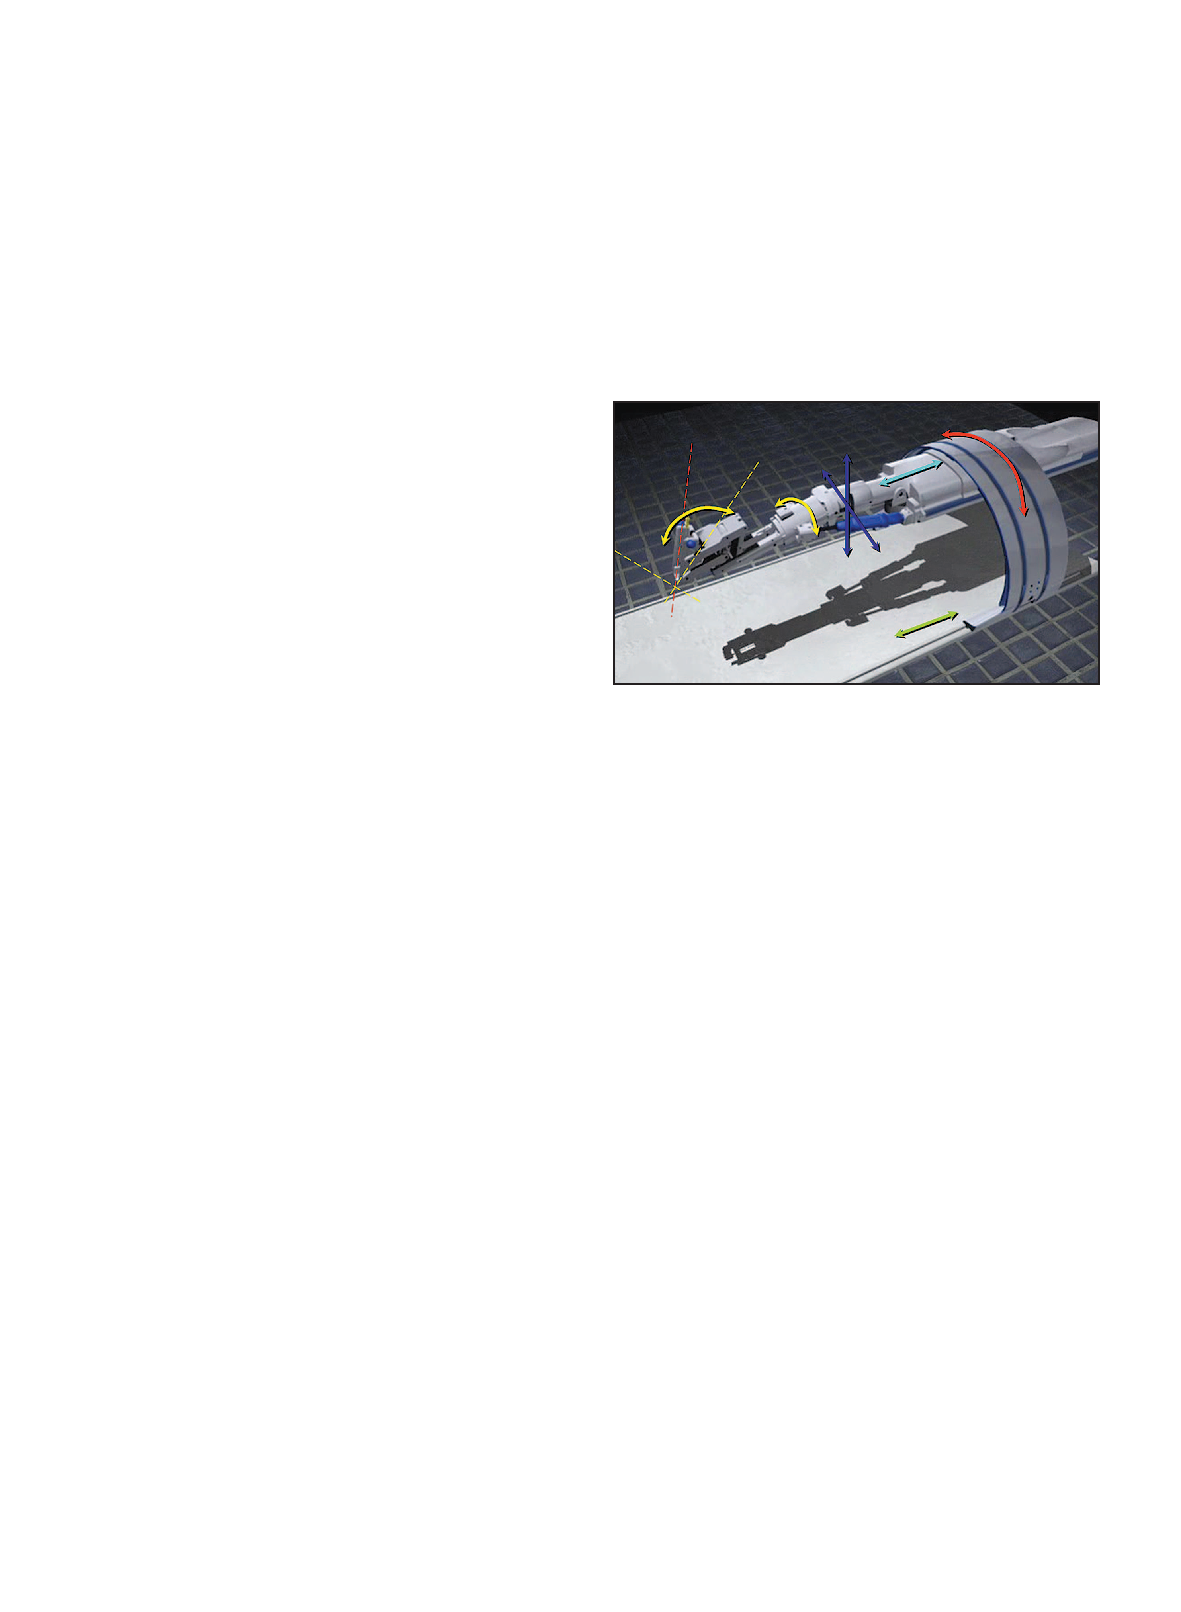
\includegraphics[width=120mm]{Fig/chap1/innomotion.pdf}
  \end{center}
  \vspace{-4mm}
\caption[CAD model of the Innomotion robotic system.]
{This is a sample figure with a sample citation \cite{Fischer2008_TMECH} \copyright 2008 IEEE.}
 \label{fig:exampleFigure}
\vspace{-2mm}
\end{figure}

\begin{table}[htb]
  \begin{center}
\caption[Scan parameters for compatibility evaluation.]{Detailed scan parameters for each of four protocols for compatibility evaluation}
\label{tab:Protocol}
  \end{center}
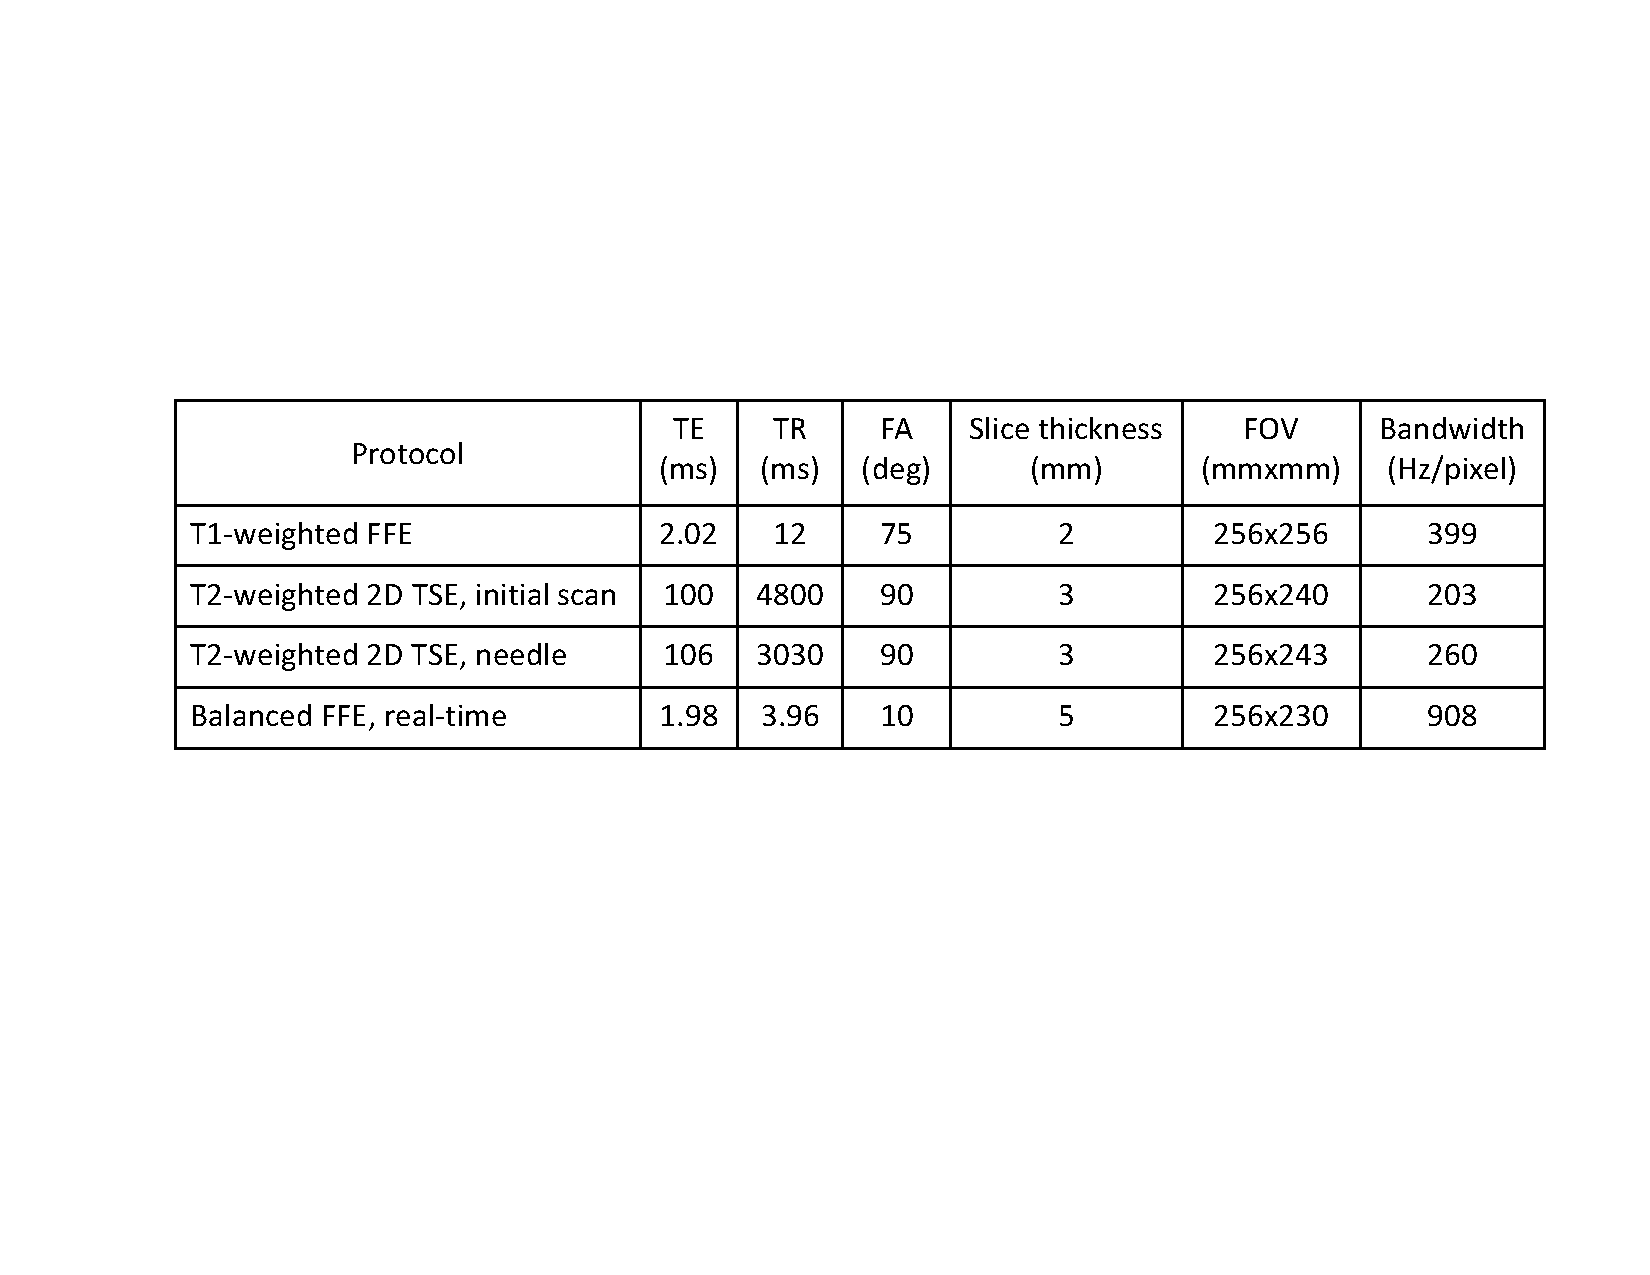
\includegraphics[width=150mm]{Fig/chap1/Protocol.pdf}
%\caption*{}
\end{table}
\vspace{-2mm}

\section{Dissertation Contributions}
\label{sec:Contributions}

\begin{itemize}
\item
\textbf{Contribution 1}

Contribution 1

\item
\textbf{Contribution 2}

Contribution 2

\item
\textbf{Contribution 3}

Contribution 3

\end{itemize}


\section{Dissertation Overview}
\label{sec:Overview}

This introductory chapter presents ...

Chapter 2 introduces ...

Chapter 3 describes ...

Chapter 4 presents ...

Chapter 5 summarizes ...

Chapter 6 presents ...

We conclude and discuss future work in Chapter 7. 